\pgfplotsset{width=7cm,compat=1.16}
\usepgfplotslibrary{polar}

\qns{Complex Numbers (Optional)}

\meta{Tell students that it's not necessary to simplify some of the values as they can be quite complicated and unwieldy. For z = a + bj, you can tell students that b is scaling j, so j acts as a unit vector for the imaginary axis. Likewise, a is multiplying an implicit "1", so it is an "invisible" unit vector for the real axis}

A complex number, $z$, is composed of a real part and imaginary part.
If $z = a + bj$, then $\mathfrak{Re}(z) = a$ (the real portion equals a), and $\mathfrak{Im}(z) = b$ (the imaginary portion equals b).
Complex numbers can be expressed in two ways:

\hspace{2 em} Rectangular Form: $z = a + bj$ \hspace{14em} Polar Form: $z = re^{j\theta}$

\begin{figure}[h]
\centering
    \begin{tikzpicture}[scale=0.8, transform shape]
    \draw (0,-4)--(0,4) node[above] {$Im$} (-4,0)--(4,0) node[right] {$Re$};
    \draw[dashed] (0,0) circle (3) circle (2) circle (1);
    \draw (-1.15,0.93)--(-1.15,1.045) node[near start, fill=white] {$r = 1$};
    \draw (-1.85,1.65)--(-1.78,1.78) node[near start=3pt, fill=white] {$r = 2$};
    \draw (-2.45,2.45)--(-2.55,2.55) node[near start=3pt, fill=white] {$r = 3$};
    \draw [line width=0.25mm, blue, ->] (0,0) -- (2.4,1.3) node [below right] {};
    \draw [dotted, line width=0.25mm, blue, ->] (0,0) -- (2.4,0) node [below right]{};
    \draw [dotted, line width=0.25mm, blue, ->] (2.4,0) -- (2.4,1.3) node [below right]{};
    \draw (1.5,-0.3)--(1.6,-0.3) node[near start=3pt, fill=white] {\color{blue}$a$};
    \draw (2.7,0.6)--(2.7,0.6) node[near start=3pt, fill=white] {\color{blue}$b$};
    \draw (3.5,1.4)--(3.5,1.4) node[near start=3pt, fill=white] {\color{blue}$z = a + bj$};
    \end{tikzpicture}
\hfill
    \begin{tikzpicture}[scale=0.8, transform shape]
    \draw (0,-4)--(0,4) node[above] {$Im$} (-4,0)--(4,0) node[right] {$Re$};
    \draw[dashed] (0,0) circle (3) circle (2) circle (1);
    \draw (-1.15,0.93)--(-1.15,1.045) node[near start, fill=white] {$r = 1$};
    \draw (-1.85,1.65)--(-1.78,1.78) node[near start=3pt, fill=white] {$r = 2$};
    \draw (-2.45,2.45)--(-2.55,2.55) node[near start=3pt, fill=white] {$r = 3$};
    \draw [line width=0.25mm, blue, ->] (0,0) -- (2.4,1.3) node [below right] {};
    \draw (3.2,1.55)--(3.2,1.55) node[near start=3pt, fill=white] {\color{blue}$z = r e^{j \theta}$};
    \draw (1.2,1.0)--(1.2,1.0) node[near start=3pt, fill=white] {\color{blue}$r$};
    \draw (0.6,0.15)--(0.6,0.15) node[scale=0.9,text opacity=1, opacity=0,near start=3pt, fill=white] {\color{blue}\small$\theta$};
    \end{tikzpicture}
\end{figure}

In polar form, $r$ represents the magnitude and $\theta$ represents the angle of the complex number with respect to the origin of the complex plane.
Rectangular form makes adding and subtracting complex numbers easier; whereas, polar form makes multiplying and dividing numbers easier.
Some handy equations to switch between forms include:

\begin{center}

\begin{tabular}{ c c c }
 $\tan(\theta) = \frac{b}{a}$ & $r = |z| = \sqrt{a^2 + b^2}$ \\ \\
 $\sin(\theta) = \frac{b}{|z|}$ & $\cos(\theta) = \frac{a}{|z|}$ \\  \\
\end{tabular}

\end{center}

\vspace{-15px}

\begin{enumerate}
\qitem \textbf{Use the formulas given above to convert between polar and rectangular form.}

\begin{enumerate}
\qitem Convert $10 + 12j$ to polar form.

\ws {
    \vspace{75px}
}

\sol{
$z = a + bj$. We can go from rectangular form to polar form by using the equation $z = |z|e^{j\theta}$, where $|z| = \sqrt{a^2 + b^2}$ and $\theta = \angle z = \atan2(b, a)$.
$$ z = 10 + 12j $$
$$ |z| = \sqrt{10^2 + 12^2} = \sqrt{244}$$
%$$ \angle z = \tan^{-1}(\frac{12}{10})$$
$$ \angle z = \atan2(12, 10)$$
$$ z = \sqrt{244}e^{j \, {\atan2(12/10)}} \approx 15.620e^{0.876j}$$
}

\qitem Convert $22e^{23j}$ to rectangular form.

\ws {
    \vspace{75px}
}

\sol{
Conversely, for $z = |z|e^{j\theta}$, we can go from polar form to rectangular form by using the equation $z = a + bj$, where $a = |z|\cos(\theta)$ and $b = |z|\sin(\theta)$. So, \\
$$ a = 22\cos(23) $$
$$ b = 22\sin(23) $$
$$ z = 22\cos(23) + 22j \sin(23) \approx -11.722 + -18.617j$$
}
\end{enumerate}


\qitem \textbf{Plot the following on a polar grid:}
\begin{enumerate}

\qitem {2}

\sol {
\newline
\begin{tikzpicture}
    \draw (0,-4)--(0,4) node[above] {$Im$} (-4,0)--(4,0) node[right] {$Re$};
    \draw[dashed] (0,0) circle (3) circle (2) circle (1);
    \draw (-1.15,0.93)--(-1.15,1.045) node[near start, fill=white] {$r = 1$};
    \draw (-1.85,1.65)--(-1.78,1.78) node[near start=3pt, fill=white] {$r = 2$};
    \draw (-2.45,2.45)--(-2.55,2.55) node[near start=3pt, fill=white] {$r = 3$};
    \draw [line width=0.25mm, blue, ->] (0,0) -- (2,0) node [below right] {2};
\end{tikzpicture}
}

\qitem {2j}

\sol {
\newline
\begin{tikzpicture}
    \draw (0,-4)--(0,4) node[above] {$Im$} (-4,0)--(4,0) node[right] {$Re$};
    \draw[dashed] (0,0) circle (3) circle (2) circle (1);
    \draw (-1.15,0.93)--(-1.15,1.045) node[near start, fill=white] {$r = 1$};
    \draw (-1.85,1.65)--(-1.78,1.78) node[near start=3pt, fill=white] {$r = 2$};
    \draw (-2.45,2.45)--(-2.55,2.55) node[near start=3pt, fill=white] {$r = 3$};
    \draw [line width=0.25mm, blue, ->] (0,0) -- (0,2) node [below right] {2j};
\end{tikzpicture}

}

\qitem {2 + 2j}

\sol {
\newline
\begin{tikzpicture}
    \draw (0,-4)--(0,4) node[above] {$Im$} (-4,0)--(4,0) node[right] {$Re$};
    \draw[dashed] (0,0) circle (3) circle (2) circle (1);
    \draw (-1.15,0.93)--(-1.15,1.045) node[near start, fill=white] {$r = 1$};
    \draw (-1.85,1.65)--(-1.78,1.78) node[near start=3pt, fill=white] {$r = 2$};
    \draw (-2.45,2.45)--(-2.55,2.55) node[near start=3pt, fill=white] {$r = 3$};
    \draw [line width=0.25mm, blue, ->] (0,0) -- (2,2) node [below right] {2 + 2j};
    \draw [dotted, line width=0.25mm, blue, ->] (0,0) -- (2,0) node [below right] {};
    \draw [dotted, line width=0.25mm, blue, ->] (2,0) -- (2,2) node [below right] {};
\end{tikzpicture}

}

\ws{
\begin{tikzpicture}
    \draw (0,-4)--(0,4) node[above] {$Im$} (-4,0)--(4,0) node[right] {$Re$};
    \draw[dashed] (0,0) circle (3) circle (2) circle (1);
\end{tikzpicture}
}

\end{enumerate}

\qitem \textbf{Calculate the magnitude and phase of the following:}
\meta {
    Clarify to students that the magnitude of a complex number is $|a + bj| = \sqrt{a^2 + b^2}$, and the phase is $\theta = \text{atan2}(a ,b)$.
}

\begin{enumerate}

\qitem {2}

\ws{
  \vspace{120px}
}

\sol {
$$z = 2 + 0j.$$
$$|z| = \sqrt{2^2 + 0^2} = 2.$$
$$\angle z = \angle 2 = 0 \, \text{rad}. $$
}

\qitem $\frac{2}{2j}$

\ws{
  \vspace{120px}
}

\sol {
$$ z = \frac{2}{2j} = (\frac{1}{j})(\frac{j}{j}) = \frac{j}{j^2} = -j = 0 - 1j.$$
$$|z| = \sqrt{0^2 + (-1)^2} = 1.$$
$$\angle z = \angle -j = \frac{3\pi}{2} \, \text{rad}.$$
}

\qitem $\frac{3j}{5}$

\ws{
  \vspace{120px}
}

\sol {
$$z = 0 + \frac{3}{5}j.$$
$$|z| = \sqrt{0^2 + \frac{3}{5}^2} = \frac{3}{5}.$$
$$\angle z = \angle \frac{3}{5}j = \frac{\pi}{2} \, \text{rad}.$$
}

\qitem $\frac{1+2j}{9+7j}$

\ws{
  \vspace{120px}
}

\sol {
$$z = \frac{1+2j}{9+7j} = \frac{z_a}{z_b}.$$
$$|z| = \frac{|z_a|}{|z_b|} = \frac{\sqrt{1^2 + 2^2}}{\sqrt{9^2 + 7^2}} = \frac{\sqrt{5}}{\sqrt{130}}. \approx 0.196.$$
$$\angle z = \angle z_a - \angle z_b = \atan2(2, 1) - \atan2(7, 9)) = 1.107 + 0.661 \approx 1.768 \, \text{rad}.$$
}

\end{enumerate}


\qitem \textbf{Show that $\frac{1}{j} = -j$.}

\ws{
  \vspace{120px}
}

\sol{
The key is to multiply the left-hand side of the equation by $\frac{j}{j}$: \\
$$\frac{1}{j} = \frac{1 * j}{j * j} = \frac{j}{j^2}$$
$$= \frac{j}{-1} = -j$$
}

\end{enumerate}

A complex number, $z = a + bj$ has a \textbf{complex conjugate}, $\overline{z} = a - bj$. In polar coordinates, the equivalent expression is $\overline{re^{j\theta}} = re^{-j\theta}$.

Note that the sum of a complex number and its conjugate is always purely real, but the difference between a complex number and its conjugate is always purely imaginary.

\begin{enumerate}[resume]

\qitem \textbf{Prove graphically that the sum of any complex number and its conjugate is always real.} \textit{Try plotting an an arbitrary complex number and its conjugate.}

\ws{
    \vspace{240px}
}

\sol{
For complex number $z = a + bj$, its conjugate is $\bar{z} = a - bj$. If we add these two together, we get $z + \bar{z} = a + bj + a - bj = 2a + 0j$. The imaginary components cancel out exactly, so the resulting sum is always entirely real. This is illustrated by the following graph for $z = 1 + 1j$ and $\bar{z} = 1 - 1j$:

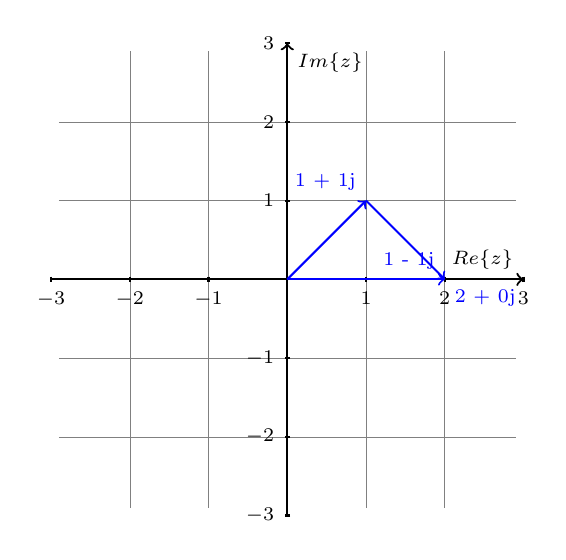
\begin{tikzpicture}
    \begin{scope}[thick,font=\scriptsize]
    \draw[step=1cm,gray,very thin] (-2.9,-2.9) grid (2.9,2.9);
    \draw [->] (-3,0) -- (3,0) node [above left]  {$Re\{z\}$};
    \draw [->] (0,-3) -- (0,3) node [below right] {$Im\{z\}$};

    \foreach \x in {-3, -2, -1, 1, 2, 3}
       \draw (\x cm,1pt) -- (\x cm,-1pt) node[anchor=north] {$\x$};
    \foreach \y in {-3, -2, -1, 1, 2, 3}
        \draw (1pt,\y cm) -- (-1pt,\y cm) node[anchor=east] {$\y$};


    \draw [line width=0.25mm, blue, ->] (0,0) -- (1,1) node [above left] {1 + 1j};
    \draw [line width=0.25mm, blue, ->] (1,1) -- (2,0) node [above left] {1 - 1j};
    \draw [line width=0.25mm, blue, ->] (0,0) -- (2,0) node [below right] {2 + 0j};
    \end{scope}
\end{tikzpicture}

}

\qitem Recall that Euler's Formula states that $e^{j\theta} = \cos(\theta) + j\sin(\theta)$.

\textbf{Using Euler's identity, show the following identities}, which show that sinusoids are sums of complex exponentials:

\begin{align*}
    \cos(\theta) = \frac{e^{j\theta} + e^{-j\theta}}{2} \\
    \sin(\theta) = \frac{e^{j\theta} - e^{-j\theta}}{2j}
\end{align*}

\sol{

  $$e^{j\theta} = \cos(\theta) + j\sin(\theta)$$

  Note that $e^{j\theta}$ has the complex conjugate $e^{-j\theta}$, which means:

  $$e^{-j\theta} = \cos(\theta) - j\sin(\theta)$$
  $$e^{j\theta} +  e^{-j\theta} = \cos(\theta) + j\sin(\theta) + \cos(\theta) - j\sin(\theta)$$
  $$e^{j\theta} +  e^{-j\theta} = 2\cos(\theta)$$
  $$cos(\theta) = \frac{1}{2}(e^{j\theta} +  e^{-j\theta})$$

  We can also notice that this is true because $cos$ is an even function and $sin$ is an odd function, which gives the properties
  $cos(-\theta) = cos(\theta)$ and $sin(-\theta) = -sin(\theta)$.

  A similar approach can be used to find $sin(\theta)$:

  \begin{align*}
    e^{j\theta} - e^{-j\theta} &= cos(\theta) + jsin(\theta) - (cos(\theta) - jsin(\theta)) \\
    &= 2jsin(\theta) \\
    \implies sin(\theta) &= \frac{e^{j\theta} - e^{-j\theta}}{2j}
  \end{align*}

}

\end{enumerate}
